In this portion of the lab we measured the sin of the phase variations of the reflected signal from the cavity. This was done by multiplying the sampled signal before it hits the cavity. 


\begin{figure}[H]
\centering
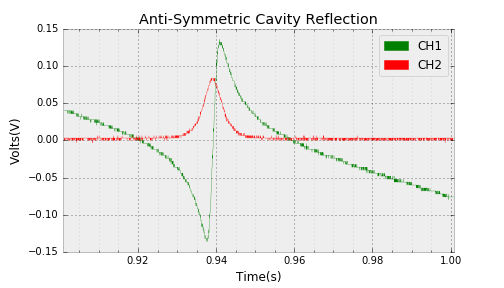
\includegraphics[width=0.75\textwidth]{figures/PartC/scope_12_raw.png}
\caption{Raw output of an anti-symmetric cavity reflection, with an interpolated voltage scale shown}
\label{fig:scope12_raw}
\end{figure}

\begin{figure}[H]
\centering
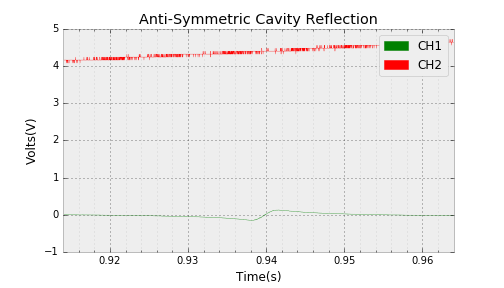
\includegraphics[width=0.75\textwidth]{figures/PartC/scope_14_raw.png}
\caption{Raw output of an anti-symmetric cavity reflection, with an interpolated voltage scale shown}
\label{fig:scope14_raw}
\end{figure}

Above we have the outputted graphs we get when scanning the VCO frequency over the resonance. The dispersion-like variation in the output of the mixer is visible.
\begin{figure}[H]
\centering
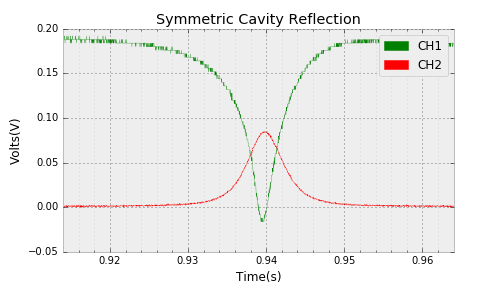
\includegraphics[width=0.75\textwidth]{figures/PartC/scope_15_raw.png}
\caption{Raw output of a symmetric cavity reflection, with an interpolated voltage scale shown}
\label{fig:scope15_raw}
\end{figure}

This is the graph of the symmetric cavity reflection. The difference between this length and the length of the trombone when looking at the Anti-Symmetric reflection is that this length is shorter than that one. 

\subsection{Additional Questions}
1. 
\begin{equation}
    |\Gamma|^2 = 1\; -\; \frac{1}{1+4 Q_\ell^2 (\Delta\omega/\omega_o)^2}
\end{equation}
\begin{equation}
    \frac{1}{Z} = \frac{1}{R} + jwC + \frac{1}{jwL}
\end{equation}
\begin{equation}
    \Gamma = \frac{Z-Z_0}{Z+Z_0}
\end{equation}
\begin{equation}
    |\Gamma|^2 = |\frac{Z-Z_0}{Z+Z_0}|^2 
\end{equation}
\begin{equation}
    |\frac{Z-Z_0}{Z+Z_0}|^2  = 1\; -\; \frac{1}{1+4 Q_\ell^2 (\Delta\omega/\omega_o)^2}
\end{equation}
\begin{equation}
   \frac{1}{1+4 Q_\ell^2 (\Delta\omega/\omega_o)^2} = 1\; -\;  \frac{(Z-Z_0)^2}{(Z+Z_0)^2}
\end{equation}
\begin{equation}
   \frac{1}{1+4 Q_\ell^2 (\Delta\omega/\omega_o)^2} = 1\; -\;  \frac{(Z-Z_0)^2}{(Z+Z_0)^2}
\end{equation}
\begin{equation}
   \frac{1}{1+4 Q_\ell^2 (\Delta\omega/\omega_o)^2} =\frac{4Z_0Z}{(Z+Z_0)^2}
\end{equation}
\begin{equation}
   1+4 Q_\ell^2 (\Delta\omega/\omega_o)^2 =\frac{(Z+Z_0)^2}{4Z_0Z}
\end{equation}
\begin{equation}
   4 Q_\ell^2 (\Delta\omega/\omega_o)^2 =\frac{(Z+Z_0)^2}{4Z_0Z} -1
\end{equation}
\begin{equation}
   4 Q_\ell^2 (\Delta\omega/\omega_o)^2 =\frac{(Z-Z_0)^2}{4Z_0Z} 
\end{equation}
\begin{equation}
   Q_\ell^2 =\frac{1}{4}\frac{(Z-Z_0)^2}{4Z_0Z} (\omega_o/\Delta\omega)^2
\end{equation}
\begin{equation}
   Q_\ell =\frac{1}{2}\frac{(Z-Z_0)}{2\sqrt{Z_0Z}} (\omega_o/\Delta\omega)
\end{equation}
Where $\Delta\omega = \frac{R}{L}$
\begin{equation}
    Q_\ell = \frac{w_0 L}{R}\frac{1}{4}\frac{(Z-Z_0)}{\sqrt{Z_0Z}}
\end{equation}

Here we have that $Z =\frac{1}{\frac{1}{R} +j\omega C+\frac{1}{j\omega L}} $

2. 
From above we see that 
\begin{equation}
    \Gamma = \frac{Z-Z_0}{Z+Z_0}
\end{equation}
With $Z =\frac{1}{\frac{1}{R} +j\omega C+\frac{1}{j\omega L}}$ from this we will then be able to compare the mixer output and the imaginary part of the Gamma function. 